\subsection{Data reduction analysis} 
\label{sec:dedup_ratio}

\paragraph{Layer sharing}

%In its  straightforward implementation Docker would not support layer sharing.
%
%Instead, every image would be a single flat archive.
%
Compared to other existing containerization frameworks~\cite{openvz}~\cite{singularity},
Docker supports the sharing of layers among different images.
%
To analyze the effectiveness of this approach, we compute how many times
each layer is referenced by images.

Figure~\ref{fig:ref_count} shows that around 90\% of layers are referenced by
a single image, an additional 5\% are referenced by 2 images, and less than
1\% of the layers are shared by more than 25 images.
%
Interestingly, there is one layer that is referenced by 184,171 images.
Further analysis reveals that this is an empty layer.
%
The presence of an empty layer in an image can be explained
by the fact that during the image build, Docker creates a new layer
for every \texttt{RUN <cmd>} instruction
in the Dockerfile~\cite{Dockerfile}.
%\NZ{I dont have dockerfile. 
%	But I checked the config files and dockerfile website. 
%	It's correct.}.
%manifests/mikahassinen-docker-whale-latest-1500714692.32.json
%
If the~\texttt{<cmd>}, which can be an arbitrary shell command,
does not modify any files in the file system,
an empty layer is created.
%
%\VT{Verify the explanation for empty layers.}
%\NZ{correct}

The next 5 top-ranked layers by reference count
are included in 29,200 -- 33,413 images.
%They are related to ubuntu, dpkg, apt, and cowsay.
Specifically, one layer contains a whole \texttt{Ubuntu 14.04.2 LTS} distribution,
one layer contains a \texttt{sources.list} file for \texttt{apt},
and one layer contains binaries and libraries needed for \texttt{dpkg}.
The other two layers are related to cowsay, a program that can generate ASCII pictures of a cow with a message~\cite{cowsay}.
One layer contains a whole installation package for \texttt{cowsay 3.03} 
while the other layer only contains the binaries for cowsay.

From the above data we can estimate that without layer sharing, the Docker Hub
dataset would grow from 47\,TB to 85\,TB, implying a \textbf{1.8$\times$} deduplication
ratio provided by layer sharing.
 
%
%\NZ{Some layer tarfiles are not easy to describe. AND. these above layers are not 
%	referred by official Ubuntu latest. Find an interesting thing: image name already
%	tells what software packages it contains.}
%

\begin{figure}[t]
	\centering
		\begin{minipage}{0.2\textwidth}
			\centering
			\includegraphics[width=1\textwidth]{graphs/shared-cnt-cdf.pdf}
			\caption{CDF of layer reference count.}
			\label{fig:ref_count}
		\end{minipage}
	\begin{minipage}{0.22\textwidth}
		\centering
		\includegraphics[width=1\textwidth]{graphs/layer-size-cdf.pdf}
		\caption{CDF of compress. and uncompress. layer size.}
		\label{fig:layer-size-cdf}
	\end{minipage}%
\end{figure}
%%		\vcomment{Figures \ref{fig:layer-size-cdf} and \ref{fig:compress-ratio}
%have different sizes, looks not neat, please fix.}
%\begin{figure}
%	\centering
%	\includegraphics[width=0.21\textwidth]{graphs/shared-cnt-cdf.pdf}
%	\caption{CDF of layer reference count.
%	}
%	\label{fig:ref_count}
%\end{figure}
%
%+-----------------------------------------------------------------------+----------------+
%|layer_id                                                               |shared_image_cnt|
%+-----------------------------------------------------------------------+----------------+
%|sha256:a3ed95caeb02ffe68cdd9fd84406680ae93d633cb16422d00e8a7c22955b46d4|184171          | empty
%|sha256:e190868d63f8f8b85b026e53b5724c3c2a4548e1d642953442559cfa5f79b2c9|33413           | ubuntu 14.04.2 LTS. 
%|sha256:909cd34c6fd77d398af1d93e9d4f7f76104903f237be3d4db7b345a19631f291|33323           | dpkg
%|sha256:0b9bfabab7c119abe303f22a146ff78be4ab0abdc798b0a0e97e94e80238a7e8|33295           | apt
%|sha256:8eed3712d2cfd8c37b19d324452ba9cdb445933c04c9175c4e945b0d7241f1e3|31517           | cowsay
%|sha256:c57b6bcc83e3e88fb3748ea3f0cb13d77c4e2ffa7b9a8ded3d636f17d2d83759|31503           | cowsay 3.03 installasion package
%|sha256:8978f6879e2f86eb7a063e70f7d89feecde9950c40fc68f1f53d00b3c8ce9b52|31179           | same cowsay but different git info
%|sha256:00bf65475aba8f1077fa9629f088a5f531d645faeccb6acd7a8626c7d896a4c4|29200           | (looks like linux distribution)

\paragraph{Compression}
%
Figure~\ref{fig:layer-size-cdf} presents compressed and uncompressed layer size
distributions.
%
We found that 50\% of the layers are smaller than 1\,MB and 90\% of the layers are
smaller than 64\,MB in compressed format.
%
If uncompressed, 50\% of the layers are smaller than 2\,MB and 90\% of the
layers are smaller than 170\,MB.
%
Moreover, the total compressed layer dataset grows from 47\,TB to 167\,TB after
decompression, resulting in a compression ratio of \textbf{3.6$\times$}.
%
Compression is complementary to layer sharing and therefore, the current registry
reduces the dataset size by a factor of \textbf{3.6$\times$1.8 = 6.5}.


\paragraph{File-level deduplication}
%
%\LR{Somewhere here we should mention that we only computed the dedup ratio
%for uncompressed data but we expect it to be similar for compressed data.}
%\NZ{addressed}
%
Next, we calculate the deduplication ratio in terms of file count and capacity for
the complete dataset.
%
After removing redundant files, there are only 3.2\% of files left that in total occupy
24\,TB, resulting in deduplication ratios of \textbf{31.5$\times$} and
\textbf{6.9$\times$} in terms of file count and capacity, respectively.
%
With compression applied, file-level deduplication can hence reduce storage utilization
by a factor of \textbf{6.9$\times$3.6 = 24.8}.
%
\begin{figure} \centering
	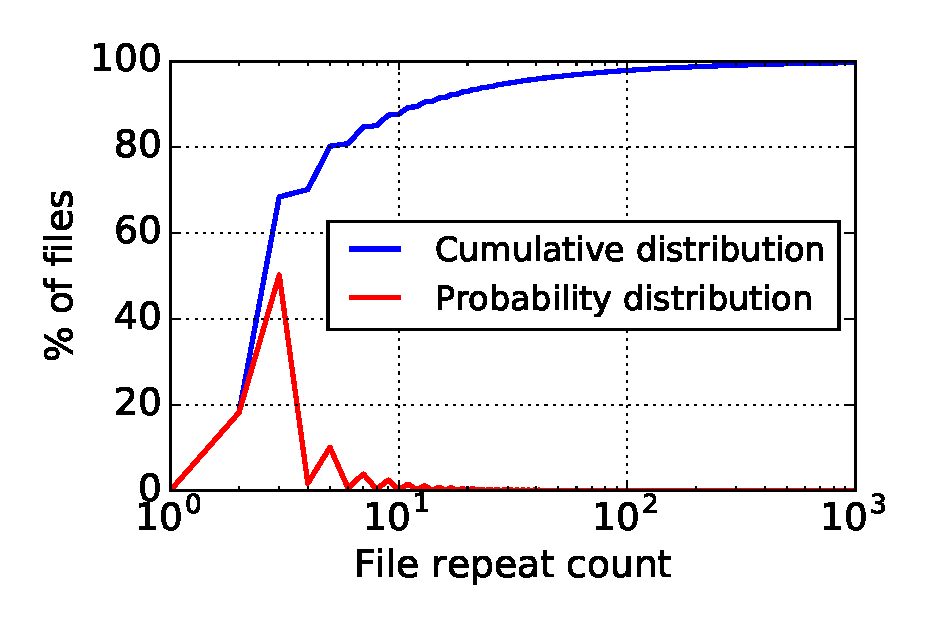
\includegraphics[width=0.45\textwidth]{graphs/File_repeat_count.eps}
	\caption{File repeat count distribution.
	%
	\VT{No need for Y2}
	%
	\VT{Still need to use \% on the axis}
	%
	} \label{fig:file-repeat-cnt}
\end{figure}


We further analyze the repeat count for every file (see Figure~\ref{fig:file-repeat-cnt}).
%
%Figure~\ref{fig:file-repeat-cnt} shows the distributions of file repeat count.  
%
We observe that over 99.4\% of files have more than one copy.
%
Around 50\% of files have exactly 4 copies and 90\% of files have 10 or less
copies. 
%
The file that has the maximum repeat count of 53,654,306 is an empty file.
%Other hot redundant files are 
%
%\VT{Do we know anything about those empty files}.\NZ{addressed}
Around 4\% of empty files are \texttt{\_\_init\_\_.py}, which make Python treat a
directory as containing packages and are usually empty.
Other frequent empty files include
\texttt{lock} or \texttt{.gitkeep} files.

We also analyze 5 frequently repeated files which repeat 3,338,145 -- 11,847,356 times.
Specifically, two files 
\texttt{libkrb5-3:amd64.postrm} and \texttt{libkrb5-3:amd64.postinst}
are two Ker\-ber\-os runtime libraries for \texttt{dpkg}.
Another two files are related to the \texttt{npm} package manager (\texttt{license} and \texttt{.npmignore})
and the last file, \texttt{dependency\_links.txt}, contains a list of dependency URLs for Python.

This shows that there is a high file-level redundancy in Docker images
which cannot be addressed by the existing layer sharing mechanism. Hence,
there is a large potential for file deduplication in the Docker registry.

\paragraph{Deduplication ratio growth}

%\begin{figure} 
%	\centering
%	\includegraphics[width=0.25\textwidth]{graphs/dedup-ratio-grow} 
%	\caption{The growth of deduplication ratio.} 
%	\label{fig:dedup-ratio-growth} 
%\end{figure}

To further study the potential of file-level deduplication, we analyze the deduplication
for an increasing number of files stored in the registry (see Figure~\ref{fig:dedup-ratio-growth}).
%
%Figure~\ref{fig:dedup-ratio-growth} shows the deduplication ratio growth over the layer dataset size.
%
The x-axis values correspond to the sizes of 4 random samples drawn from the whole dataset and the size of the
whole dataset.

We see that the deduplication ratio increases almost linearly with the layer dataset size.
%
In terms of file count, it increases from \textbf{3.6$\times$} to \textbf{31.5$\times$} while
in terms of capacity, it increases from \textbf{1.9$\times$} to
\textbf{6.9$\times$} as the layer dataset grows from 1000 to 1.7 million layers.
%
This confirms the high potential for file-level deduplication in large-scale
Docker registry deployments.
%
%As the number of images stored in the Docker registry increases dramatically,
%file-level deduplication can provide significant storage space savings.
